\chapter{Background}
\lhead{\emph{Background}}
\section{Telerobotics}
\section{Virtual Reality}
\subsection{Unreal Engine 4}
\section{Data Abstraction}

"Data abstraction" is the phrase that will be used in this report to describe the act of reducing an image down to only its most essential elements. It is similar in concept to an artist sketching a scene as opposed to attempting a full drawing, and is comparable to data compression as the aim is also to reduce the file size of the image, however data abstraction takes a very different approach to solving the problem than standard compression algorithms.

Data compression is the storing of information using a more space efficient encoding \cite{compression}. While some information is lost during lossy compression, the aim regardless of the algorithm used is to retain as much of the original information as possible. In contrast, the aim when utilising data abstraction is to discard all the information that is unnecessary to fulfilling the image's purpose. For example, if all that is required of a image is that basic shapes can be identified, then only the information on the boundaries of the shapes is necessary; the rest of the image can be discarded. An implementation of data abstraction can be seen in Figure \ref{fig:abstraction3rdyear}.

%\caption[My figure Title.]{My figure Title. Details how it was made. What is the point? Reproduced from}

\begin{figure}[H]
    \begin{center}
      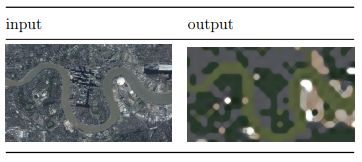
\includegraphics[width=0.6\textwidth]{Figures/abstraction3rdyear.png}
      \caption[Data Abstraction Example]{Data Abstraction Example. This is the abstraction of an aerial photograph of London, reproduced from \cite{abstraction3rdyear}}
      \label{fig:abstraction3rdyear}
    \end{center}
\end{figure}

\section{Inter-Frame Interpolation}

\section{Sobol Sequences}

Sobol sequences are quasi-random sequences that were introduced to aid in approximating integrals over an S-dimensional unit cube \cite{joe2008constructing}. The aim is to form a sequence $x_i$ in S-dimensional unit cube $I^S$ that approximates
\begin{equation}
    \int_{I^S} f \quad by \quad \lim_{n\to\infty}\frac{1}{n}\sum_{i=1}^{n} f(x_i)
\end{equation}
For this to hold, the points of $x_i$ should be selected so they are evenly spread across $I^S$. This provides a much more even spread of points across the chosen space than can be produced from a pseudo-random number source (Figure \ref{fig:Sobol}). The code used in this project to produce these sequences was created by Leonhard Gr\"unschlo\ss\space \cite{CodeSource} \textcolor{red}{and is presented in Appendix A.}

\begin{figure}[H]
    \begin{center}
    \begin{tabular}{ c c }
        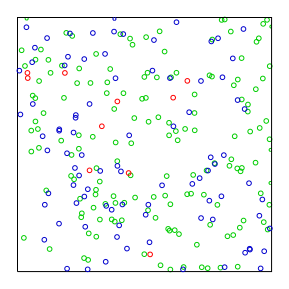
\includegraphics[width=0.33\textwidth]{Figures/Pseudorandom_sequence_2D.png} &
        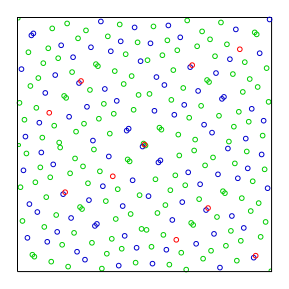
\includegraphics[width=0.33\textwidth]{Figures/Sobol_sequence_2D.png}
    \end{tabular}
    \caption[Comparison of pseudo-random and quasi-random sequences]{Comparison of pseudo-random and quasi-random sequences. 256 points from a pseudo-random generator (left) and 256 points from a Sobol sequence (right), reproduced from \cite{SobolWiki}.}
    \label{fig:Sobol}
    \end{center}
\end{figure}

\section{Computer Vision}

Computer vision is the automatic analysis of images and extraction of the useful information they contain \cite{CVDef}. A raw image is simply a large matrix of colour values, so for a computer to take action based on the contents of an image it must be able to recognise features using analysis of this data. Doing so involves many different techniques such as statistical pattern classification and geometric modelling \cite{ballard1982computer}. All computer vision methods in this project are implemented using the OpenCV libraries, and the example programs provided with them used as starting points for development \cite{OpenCV}.

\subsection{Edge Detection}
When attempting to recognise the features of an image, knowing the locations of the edges of objects within the scene is often very useful. An edge is defined as a significant local change in intensity, usually due to a discontinuity in either the intensity or its first derivative \cite{jain1995machine}. There are many algorithms available that will detect the edges of an image from the locations of these discontinuities. When the most popular algorithms (Laplacian of Gaussian, Robert, Prewitt, Sobel, and Canny) are compared, the most effective in almost all scenarios is Canny edge detection \cite{maini2009study}, therefore this is the algorithm utilised in this project. Canny edge detection \cite{canny1986computational} (Figure \ref{fig:canny1}), \textcolor{red}{and can be divided into 4 stages:}
\begin{enumerate}
    \item \textcolor{red}{Reduce noise using a Gaussian filter}
    \item \textcolor{red}{Find the intensity gradient of the image by taking the first derivative in the horizontal and vertical directions.}
    \item \textcolor{red}{Remove from the gradient map any pixel that is not a local maximum, reducing the edges down to their minimum thickness.}
    \item \textcolor{red}{Remove any edge that either has an intensity gradient lower than a lower threshold value or not connected to pixels with a value larger than an upper threshold value (hysteresis thresholding).}
\end{enumerate}

\begin{figure}[H]
    \begin{center}
      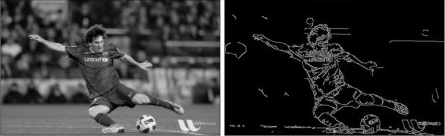
\includegraphics[width=0.9\textwidth]{Figures/canny2.png}
      \caption[Canny Edge Detection Example]{Canny Edge Detection Example. Simple edge detection program applied to a fairly detailed photo of Messi, to demonstrate its effectiveness even with more complex images. Figure taken from an OpenCV Canny tutorial \cite{Canny1Source}.}
      \label{fig:canny1}
    \end{center}
\end{figure}

\subsection{Flood Fill}

Flood fill algorithms determine the area connected to a given cell (the seed point) in a multi-dimensional array that have similar intensity values for the purpose of filling them with a chosen colour \cite{FloodFill}. This is a technique that is not only useful in image processing, but also for many other fields such as in passive acoustic monitoring where finding the area connected to a given node can be useful as part of tracking in 4D space (x,y,z,time) \cite{nosal2008flood}. A demonstration of flood fill has been presented in Figure \ref{fig:EgFloodFill}.

\begin{figure}[H]
    \begin{center}
    \begin{tabular}{ c c }
        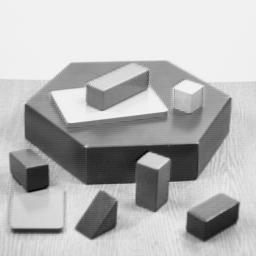
\includegraphics[width=0.35\textwidth]{Figures/blox.jpg} &
        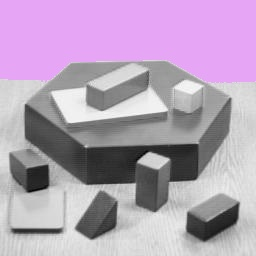
\includegraphics[width=0.35\textwidth]{Figures/bloxFilled.jpg}
    \end{tabular}
    \caption[Example of Flood Fill]{Example of Flood Fill. The original image (left) was provided by OpenCV. The right image is the result of flood filling from the top left corner, filling the lighter space at the back of the scene.}
    \label{fig:EgFloodFill}
    \end{center}
\end{figure}

\subsection{Depth Mapping}

\section{Image Compression}

\section{UDP Communications}